% REVISÃO BIBLIOGRÁFICA------------------------------------------------------------------

\chapter{REVISÃO DE LITERATURA}
\label{chap:revisao_bibliografica}
\section{Objetivos de desenvolvimento sustentável}

\lipsum[13-15]

\section{Álcoois e Ácidos  carboxílicos}

\begin{citacao}
	\lipsum[16] \cite{Barbosa2012}
\end{citacao}

\lipsum[16-17] \cite{Barbosa2012}

\lipsum[18-19] \cite{Hoekman2012}.

\begin{table}[H]
    \centering
    \caption{Grupos de ácidos graxos típicos em biodiesel}
    \begin{tabular}{lccc}
    \hline
    Nome & N$^0$ CAS  & Fórmula Molecular  & Estrutura Molecular  \\
    \hline
    Ácido Láurico & 143-07-7 & \ch{C12H24O2} & \raisebox{-0.5\height}{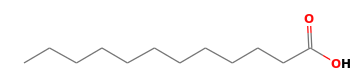
\includegraphics[width=0.4\linewidth]{dados/figuras/Ac_laurico.png}} \\
    Ácido Miristico & 544-63-8 & \ch{C14H28O2} & 
    \end{tabular}
    \label{tab:Grupo}
\end{table}

\lipsum[20-21] \cite{Fonseca2005}.
    
\lipsum[22-25]
\begin{table}[H]
\centering
\caption{Composição dos ácidos graxos do óleo de soja, de rícino e de cambre.}
\begin{tabular}{lp{2.5cm}p{2.5cm}p{2.5cm}}
\hline
\multirow{2}{*}{Nomenclatura do Ácido} & \multicolumn{3}{l}{Porcentagem de ácidos carboxílicos totais (\%)}  \\
    & Soja  & Rícino & Crambe  \\
    \hline
     Ácido Láurico      & 0,1 (máx.)  &  & \\
     Ácido Mirístico    & 0,2 (máx.)  &  &  \\
     Ácido Palmítico    & 9,9 - 12,2  & 0,9 -1,5 & 3,4  \\
     Ácido Palmitoléico & Traços -0,2 &  &  \\
     Ácido Esteárico    & 3 - 5,4     & 1,4-2,1  & 1,1 \\
     Ácido Oleico       & 17,7 - 26   & 3,1-5,9 & 17,8 \\
     Ácido Linoléico    & 49,7 - 56,9 & 2,9- 6,5 & 6,1 \\
     Ácido Linolênico   & 5,5 - 9,5   &  & 2,8 \\
     Ácido Araquídico   & 0,2 - 0,5   &  & 1,7 \\
     Ácido Gadolêico    & 0,1 - 0,3   &  &  \\
     Ácido Behênico     & 0,3 - 0,7   &  & 3,7 \\
     Ácido Erúcico      & 0,3 (máx.)  &  & 56,7 \\
     Ácido Lignocérico  & 0,4 (máx.)  &  &  \\
     Ácido Eicosenóico  &             &  & 6,7 \\
     Ácido Ricinoléico  &             & 84,0 -91,0 &  \\
     \hline
\end{tabular}
\label{tab:angelica}
\end{table}

\section{Equilíbrio de fases sólido-líquido}
	
\lipsum[13-15] \cite{Prausnitz}
	
	%Número de propriedades intensivas = número de componentes - número de fases +2

	\begin{description}
		\item[i)] número de mol deve ser um valor positivo:
		\begin{equation}
		\eta_{ij}\geqslant 0,\  \ i=1,2,\ldots,NC \mbox{ e } j=1,2,\ldots,NF
		\end{equation}
		\item[ii)] conservação de massa sem reações químicas:
		\begin{equation}
		\sum_{i=1}^{NC}\eta_{ij}=\eta_{i},\  \ i=1,2,\ldots,NC
		\end{equation}
	\end{description}
	em que $\eta_{i}$ é número total de mols do componente $i$.
	\cite{Sandlel,Barbosa2012,Prausnitz}
	
	\section{Cálculo do equilíbrio para substância pura}
	
	\hspace{5mm} 
	
	\lipsum[13-15]
	\begin{equation}\label{eq:atividade_1}x_i=\frac{f_{i(\mbox{\tiny sólido puro})}}{\gamma_{i}f_{i(\mbox{\tiny líquido sub-resfriado puro})}}
	\end{equation}
	para simplificar a notação
	\begin{equation*}
	f_{i}^{S}=f_{i(\mbox{\tiny sólido puro})}
	\end{equation*}
	e
	\begin{equation*}
	f_{i}^{L}=f_{i(\mbox{\tiny líquido sub-resfriado puro})}
	\end{equation*}
	
	\lipsum[13-15]

	\subsection{Ácido Mirístico}
	\label{sec:1}
	\begin{itemize}
		\item Estrutura
		\begin{figure}[H]
			\centering
			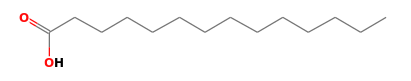
\includegraphics[width=0.7\linewidth]{dados/figuras/Ac_miristico.png}
			\caption[Ácido Mirístico]{Ácido Mirístico  NIST \textit{National Institute of Standards and Technology}}
			\label{fig:nist1}
		\end{figure}
		\item Número do CAS: 544-63-8
		\item Fórmula Molecular: \ch{C14H28O2}
		\item Temperatura de fusão ($T_f$)=327.55 k
		\item Entalpia ($\Delta H_{f}$)=10.771955 kcal/mol
	\end{itemize}
	
	\subsection{Ácido Esteárico}
	\label{sec:2}
	\begin{itemize}
		\item Estrutura
		\begin{figure}[H]
			\centering
			\includegraphics[width=0.7\linewidth]{dados/figuras/Ac_estearico.png}
			\caption[Ácido Esteárico]{Ácido Esteárico NIST \textit{National Institute of Standards and Technology}}
			\label{fig:nist2}
		\end{figure}
		\item Número do CAS: 57-11-4
		\item Fórmula Molecular: \ch{C18H36O2}
		\item Temperatura de fusão ($T_f$)=342.75 k
		\item Entalpia ($\Delta H_{f}$)=14.64126 kcal/mol
	\end{itemize}
	
	\subsection{Ácido Palmítico}
	\label{sec:3}
	\begin{itemize}
		\item Estrutura
		\begin{figure}[H]
			\centering
			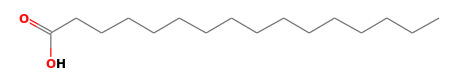
\includegraphics[width=0.65\linewidth]{dados/figuras/Ac_palmitico.png}
			\caption[Ácido Palmítico]{Ácido Palmítico NIST \textit{National Institute of Standards and Technology}}
			\label{fig:nist3}
		\end{figure}
		\item Número do CAS: 57-10-3
		\item Fórmula Molecular: \ch{C16H32O2}
		\item Temperatura de fusão ($T_f$)=336.00 k
		\item Entalpia ($\Delta H_{f}$)=80.252256 kcal/mol
	\end{itemize}
	
	\subsection{1-Hexadecanol}
	\label{sec:4}
	\begin{itemize}
		\item Estrutura
		\begin{figure}[H]
			\centering
			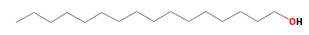
\includegraphics[width=0.8\linewidth]{dados/figuras/Hexadecanol.png}
			\caption[1-Hexadecanol]{1-Hexadecanol NIST \textit{National Institute of Standards and Technology}}
			\label{fig:8}
		\end{figure}
		\item Número do CAS: 36653-82-4
		\item Fórmula Molecular:\ch{C16H34O}
		\item Temperatura de fusão ($T_f$)=322,35k
		\item Entalpia ($\Delta H_{f}$)=8.025226 kcal/mol
	\end{itemize}
	


	